\documentclass[12pt]{article}
\usepackage{graphicx}
\usepackage[margin=1in]{geometry}
\usepackage{amsmath, amssymb} 
\usepackage{listings} 
\usepackage{xcolor} 

\lstset{
    basicstyle=\ttfamily,
    columns=fullflexible,
    frame=single,
    breaklines=true,
    postbreak=\mbox{\textcolor{red}{$\hookrightarrow$}\space},
}

\title{Mathematical Morphology Operations on Binary Images}
\author{Matteo Scardovi}
\date{\today}

\begin{document}

\maketitle

\section{Program Overview}
This report discusses a Python program designed to perform mathematical morphology operations on images. These operations include erosion, dilation, opening, and closing.

The program is implemented in Python, utilizing libraries such as OpenCV for image reading and manipulation, NumPy for efficient array operations, and Matplotlib for displaying images. 

It accepts an image and a structuring element as input, along with the desired morphological operation to perform: erosion (`e`), dilation (`d`), opening (`o`), or closing (`c`). The program then applies the specified operation to the image using the structuring element and displays the original and processed images side by side.

\section{Morphological Operations}
\subsection{Erosion}
Erosion shrinks bright regions and enlarges dark regions, effectively eroding the boundaries of the foreground object. It is used to remove small white noises from images or to detach two connected objects.

\subsection{Dilation}
Dilation, in contrast to erosion, adds pixels to the boundaries of objects in an image, increasing object areas and accentuating features.

\subsection{Opening}
Opening is an erosion followed by a dilation. It is used to remove small objects from the foreground of an image, smoothing the contours of objects, and eliminating thin protrusions.

\subsection{Closing}
Closing is a dilation followed by an erosion. It is useful in closing small holes inside the foreground objects or small black points on the object.

\section*{Usage}

To use the program, you must provide three arguments to the command line: the path to the image file, the path to the structuring element image file, and the operation to be performed.

\begin{verbatim}
python MorphOps.py [image_path] [structuring_element_path] [operation]
\end{verbatim}

\begin{itemize}
    \item \textbf{image\_path}: Required. The path to the image file on which the morphological operation will be performed.
    \item \textbf{structuring\_element\_path}: Required. The path to the binary image file that represents the structuring element.
    \item \textbf{operation}: Required. Specifies the morphological operation to perform. Use `e' for erosion, `d' for dilation, `c' for closing, and `o' for opening.
\end{itemize}

\section*{Examples}
\subsection{Erosion}
\begin{verbatim}
    python MorphOps.py sea.png 5x5.png e
\end{verbatim}
\begin{figure}[h!]
    \centering
    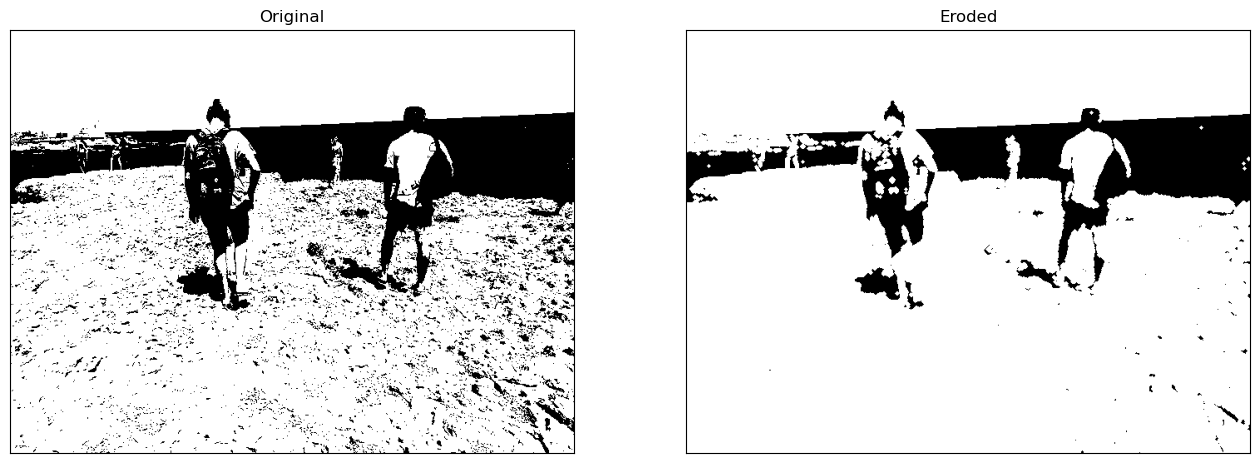
\includegraphics[width=0.9\textwidth]{erosion.png}
    \caption{Eroded image with a 5x5 structuring element.}
\end{figure}
\newpage
\subsection{Dilation}
\begin{verbatim}
    python MorphOps.py sea.png 5x5.png d
\end{verbatim}
\begin{figure}[h!]
    \centering
    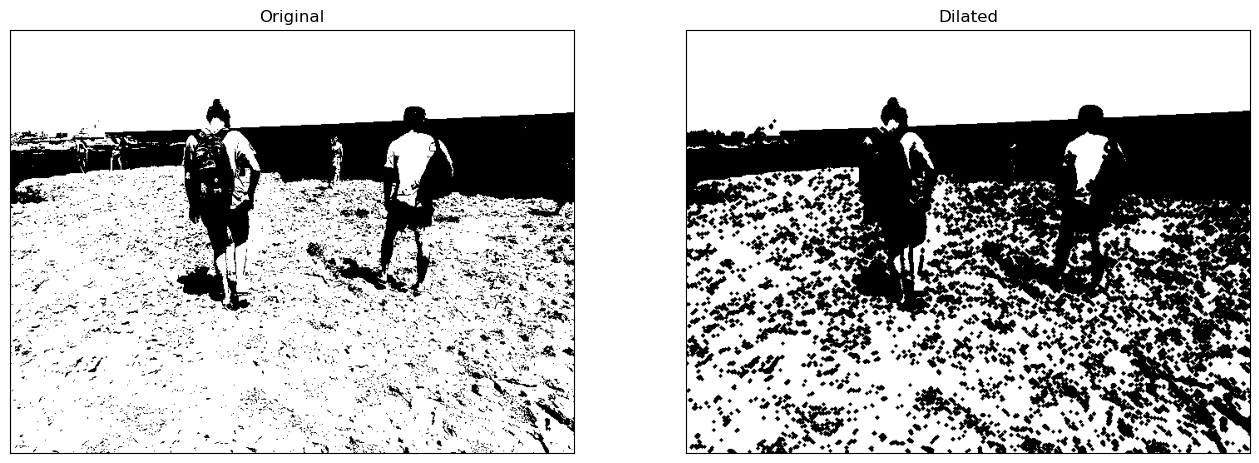
\includegraphics[width=0.9\textwidth]{dilation.png}
    \caption{Dilated image with a 5x5 structuring element.}
\end{figure}

\subsection{Opening}
\begin{verbatim}
    python MorphOps.py sea.png 5x5.png o
\end{verbatim}
\begin{figure}[h!]
    \centering
    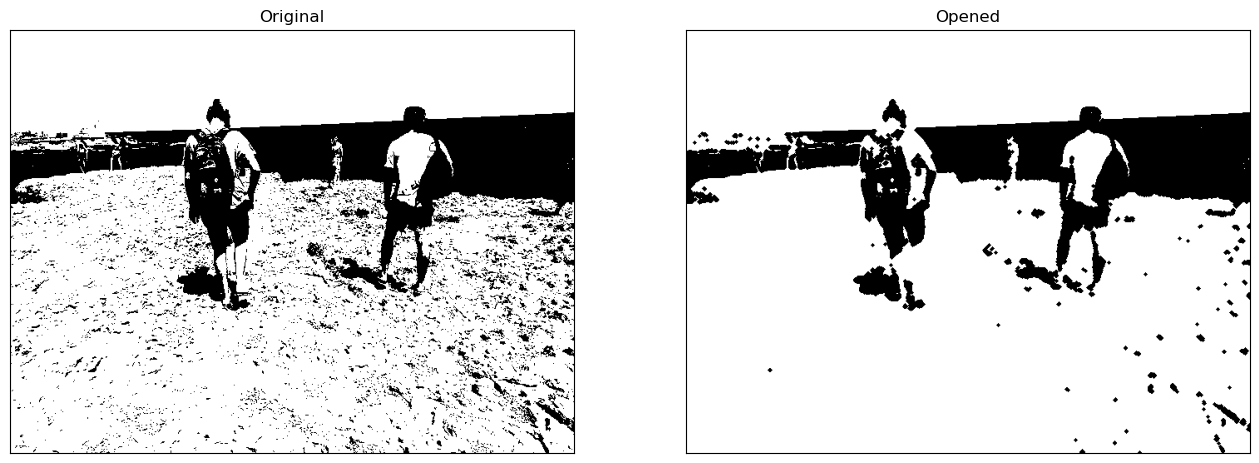
\includegraphics[width=0.9\textwidth]{opening.png}
    \caption{Opened image with a 5x5 structuring element.}
\end{figure}
\newpage
\subsection{Closing}
\begin{verbatim}
    python MorphOps.py sea.png 5x5.png c
\end{verbatim}
\begin{figure}[h!]
    \centering
    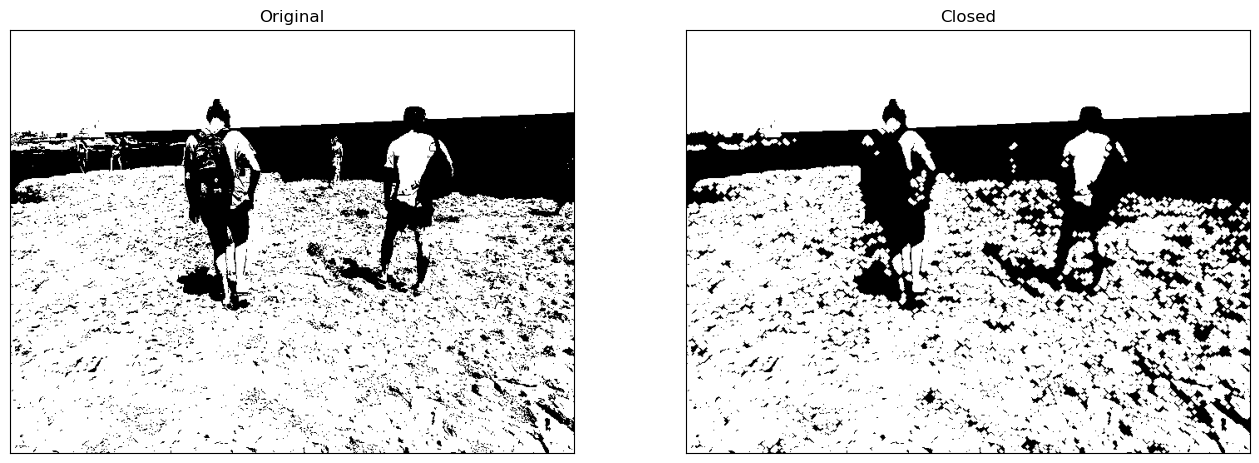
\includegraphics[width=0.9\textwidth]{closing.png}
    \caption{Closed image with a 5x5 structuring element.}
\end{figure}


\end{document}
